\section{Exercise 4}

An e-commerce web application manages data about catalogs of articles belonging to different brands and categories. 
After logging in, the user can access a HOME page where he can start to drill down the catalog. 
In the HOME page, he can select one category (e.g., "sports apparel") from a list of categories to see its brands, which are shown in a brands page. 
For the list of brands in the brands page, he can select one brand (e.g., "Adidas") of the chosen category to see its articles, which are listed in an articles page.
By choosing one article from the list in the articles page he can see the details of the chosen article in the article page. 
The details of an article include: code, name, price, picture and the brand it belongs to.
Clicking on the brand attribute of an article leads back to the articles page showing all the articles of that brand. 
When a user displays the details of an article, the application creates a relationship between the user and the article's brand, to record that the user may have a preference for such a brand.
The categories are in the order of tens, the brands in the order of hundreds, and the articles in the order of hundreds of thousands. 

Write the entity classes of the ORM mapping, including annotations for the attributes and for the relationships, fetch type of attributes and of relationships, and operation cascading policies for relationships (when not by default). 
Motivate the design choices. 
Specify the named queries used by the methods of the business objects.
\begin{figure}[H]
    \centering
    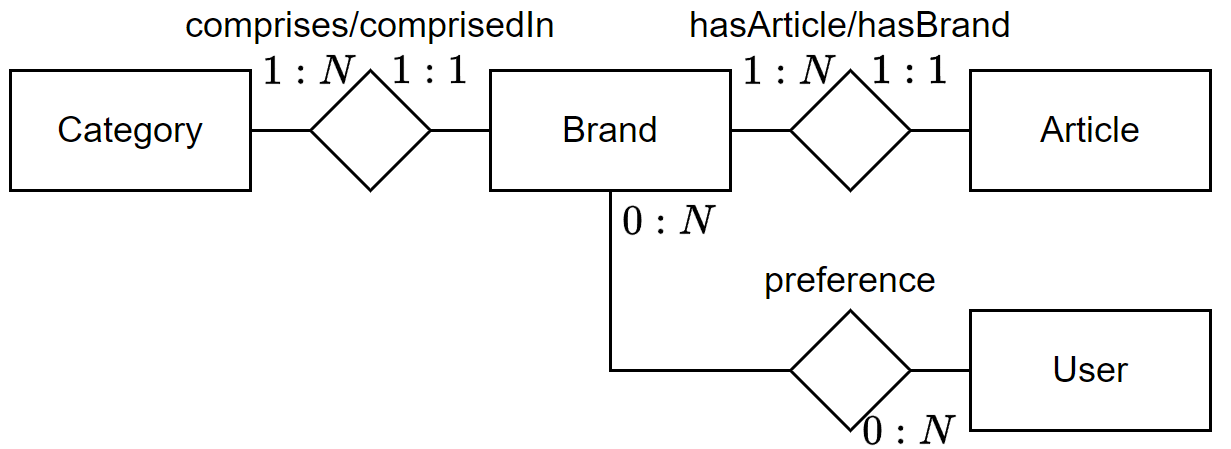
\includegraphics[width=0.75\linewidth]{images/jpa1.png}
\end{figure}

\subsection*{Solution}
We start by checking all the relationships in the E-R diagram: 
\begin{itemize}
    \item Comprises/comprisedIn: from category to brand we have to use the annotations: 
        \begin{lstlisting}[style=Java]
@OneToMany
FetchType.EAGER
        \end{lstlisting}
        Note that remove can be cascaded. 
        From brand to category we have to use these annotations: 
        \begin{lstlisting}[style=Java]
// This annotation can be omitted since it is implicit
@ManyToOne
        \end{lstlisting}
        The owner of the relation is brand. 
    \item Articles/hasBrand: from brand to article we have to use the annotations: 
        \begin{lstlisting}[style=Java]
@OneToMany
FetchType.LAZY
        \end{lstlisting}
        Note that remove can be cascaded. 
        From article to brand we have to use these annotations: 
        \begin{lstlisting}[style=Java]
@ManyToOne
        \end{lstlisting}
        The owner of the relation is article. 
    \item Preference: from user to brand we have to use the annotations: 
        \begin{lstlisting}[style=Java]
@ManyToMany
FetchType.EAGER
        \end{lstlisting}
        From brand to user we have to use these annotations: 
        \begin{lstlisting}[style=Java]
// This annotation can be omitted
@ManyToOne
FetchType.LAZY
        \end{lstlisting}
        The owner of the relation can be either user or brand. 
\end{itemize}
We can now define the four entity mappings. 
The entity category is defined as:  
\begin{lstlisting}[style=Java]
@Entity
public class Category{

    @Id @GeneratedValue(strategy=GenerationType.AUTO)
    private int categoryId;
    private String categoryName;

    @OneToMany(mappedBy="category", fetch = FetchType.EAGER,
    cascade = CascadeType.REMOVE)
    private List<Brand> brands;
    ...
}
\end{lstlisting}
The entity brand is defined as:  
\begin{lstlisting}[style=Java]
@Entity
public class Brand {

    @Id @GeneratedValue(strategy=GenerationType.AUTO)
    private int brandId;
    private String brandName;

    @ManyToOne
    @JoinColumn(name="category")
    private Category category;

    @OneToMany(mappedBy="brand", fetch = FetchType.LAZY,
    cascade=CascadeType.REMOVE)
    private List<Article> articles;

    @ManyToMany(fetch = FetchType.LAZY)
    @JoinTable( name="usr_brand", joinColumns={
                @JoinColumn(name="brandid")}, 
                inverseJoinColumns={@JoinColumn(name="userid")})
    private List<User> interestedUsers;
    ...
}
\end{lstlisting}
The entity article is defined as:  
\begin{lstlisting}[style=Java]
@Entity
public class Article{

    @Id @GeneratedValue(strategy=GenerationType.AUTO)
    private int articleId;
    private String articleCode;
    private String articleName;
    private double price;

    @Basic(fetch = FetchType.LAZY) @Lob
    private byte[] picture;

    @ManyToOne
    @JoinColumn(name="brand")
    private Brand brand;
    ...
}
\end{lstlisting}
The entity user is defined as:  
\begin{lstlisting}[style=Java]
@Entity
public class User implements Serializable {

    @Id
    @GeneratedValue(strategy = GenerationType.IDENTITY)
    private String password;
    private String username;

    @ManyToMany(mappedBy = "interestedUsers", fetch = FetchType.EAGER)
    private List<Brand> preferredBrands;
    ...
}
\end{lstlisting}